\documentclass[11pt,a4paper]{article}
\usepackage[utf8]{inputenc}
\usepackage[T1]{fontenc}
\usepackage{amsmath,amssymb,amsfonts}
\usepackage{booktabs}
\usepackage{graphicx}
\usepackage[margin=2.5cm]{geometry}
\usepackage{hyperref}
\usepackage{float}
\usepackage{caption}
\usepackage{xcolor}
\usepackage{multirow}

\title{1D Anisotropic XYZ Spin Ring:\\Trotterized Hamiltonian Simulation \& Spectral Analysis\\on IBM Quantum Hardware}
\author{Hackathon Team}
\date{\today}

\begin{document}
\maketitle

\begin{abstract}
We present a digital quantum simulation of the 1D anisotropic XYZ Heisenberg model with periodic boundary conditions on $N=4$ qubits. 
The time evolution operator $e^{-i\hat{H}t}$ is approximated via Lie-Trotter (1st order), Suzuki-Trotter (2nd order), and Suzuki-Trotter (4th order) decompositions. 
We compare simulation results across three execution tiers---noiseless statevector, noisy simulation (FakeBrisbane), and real quantum hardware (\texttt{ibm\_yonsei})---against exact diagonalization. 
Error mitigation through Dynamic Decoupling (DD, XY4 sequence) and Twirled Readout Error eXtinction (TREX) is evaluated.
Energy gap information is extracted via FFT spectral analysis of the time-dependent magnetization signal.
\end{abstract}

% =====================================================
\section{Model Hamiltonian \& Initial State}
% =====================================================

The 1D periodic anisotropic XYZ Hamiltonian on $N=4$ qubits with transverse field is:
\begin{equation}
    \hat{H} = \sum_{i=0}^{N-1} \left( J_x\, X_i X_{i+1 \bmod N} + J_y\, Y_i Y_{i+1 \bmod N} + J_z\, Z_i Z_{i+1 \bmod N} \right) + h \sum_{i=0}^{N-1} Z_i
\end{equation}
with coupling constants $J_x = 1.0$, $J_y = 0.8$, $J_z = 0.5$, and transverse field $h = 0.5$.

The coupling topology is a \textbf{ring} (periodic boundary conditions), so the bond set is $\{(0,1), (1,2), (2,3), (3,0)\}$.

The initial state is the antiferromagnetic N\'eel state:
\begin{equation}
    |\psi(0)\rangle = |0101\rangle
\end{equation}

The tracked observable is the single-site magnetization:
\begin{equation}
    \langle Z_0(t) \rangle = \langle\psi(t)| Z_0 \otimes I^{\otimes 3} |\psi(t)\rangle
\end{equation}

% =====================================================
\section{Exact Diagonalization}
% =====================================================

Exact diagonalization of $\hat{H}$ yields the energy spectrum shown in Table~\ref{tab:eigenvalues}.

\begin{table}[H]
\centering
\caption{Complete energy spectrum of the 4-qubit XYZ Hamiltonian.}
\label{tab:eigenvalues}
\begin{tabular}{cc|cc}
\toprule
$n$ & $E_n$ & $n$ & $E_n$ \\
\midrule
$0$ & $-6.205224$ & $1$ & $-4.677033$ \\
$2$ & $-2.522967$ & $3$ & $-2.000000$ \\
$4$ & $-1.000000$ & $5$ & $-1.000000$ \\
$6$ & $-0.012296$ & $7$ & $-0.000000$ \\
$8$ & $-0.000000$ & $9$ & $0.000000$ \\
$10$ & $1.000000$ & $11$ & $1.000000$ \\
$12$ & $2.522967$ & $13$ & $3.783783$ \\
$14$ & $4.433737$ & $15$ & $4.677033$ \\
\bottomrule
\end{tabular}
\end{table}

Key spectral properties:
\begin{itemize}
    \item Ground state energy: $E_0 = -6.205224$
    \item First excited state energy: $E_1 = -4.677033$
    \item Spectral gap: $\Delta E_{01} = E_1 - E_0 = 1.528191$
\end{itemize}

\subsection{Initial State Decomposition}

The N\'eel state overlap with energy eigenstates determines which energy differences appear in the time evolution.
Only states with non-negligible overlap $| \langle E_n | \psi(0) \rangle |^2 > 10^{-4}$ contribute:

\begin{table}[H]
\centering
\caption{Significant overlaps of the N\'eel state with energy eigenstates.}
\label{tab:overlaps}
\begin{tabular}{ccc}
\toprule
$n$ & $E_n$ & $| \langle E_n | \psi(0) \rangle |^2$ \\
\midrule
$0$ & $-6.205224$ & $0.296537$ \\
$3$ & $-2.000000$ & $0.500000$ \\
$6$ & $-0.012296$ & $0.003078$ \\
$13$ & $3.783783$ & $0.074382$ \\
$14$ & $4.433737$ & $0.126004$ \\
\bottomrule
\end{tabular}
\end{table}

The dominant energy differences driving the time evolution of $\langle Z_0(t) \rangle$ are:

\begin{table}[H]
\centering
\caption{Dominant energy differences and corresponding frequencies.}
\label{tab:energy_diffs}
\begin{tabular}{ccc}
\toprule
$\Delta E$ (a.u.) & $\omega = \Delta E$ (rad/s) & $f = \omega / 2\pi$ (Hz) \\
\midrule
$0.523$ & $0.523$ & $0.083$ \\
$0.650$ & $0.650$ & $0.103$ \\
$0.893$ & $0.893$ & $0.142$ \\
$0.988$ & $0.988$ & $0.157$ \\
$1.000$ & $1.000$ & $0.159$ \\
$1.528$ & $1.528$ & $0.243$ \\
\bottomrule
\end{tabular}
\end{table}

% =====================================================
\section{Trotterization}
% =====================================================

The time-evolution operator is approximated using product formulas:

\subsection{Lie-Trotter (1st order)}
\begin{equation}
    e^{-i(A+B)t} \approx \left( e^{-iA\frac{t}{r}} e^{-iB\frac{t}{r}} \right)^r + \mathcal{O}\left(\frac{t^2}{r}\right)
\end{equation}

\subsection{Suzuki-Trotter (2nd order)}
\begin{equation}
    e^{-i(A+B)t} \approx \left( e^{-iA\frac{t}{2r}} e^{-iB\frac{t}{r}} e^{-iA\frac{t}{2r}} \right)^r + \mathcal{O}\left(\frac{t^3}{r^2}\right)
\end{equation}

\subsection{Suzuki-Trotter (4th order)}
\begin{equation}
    S_4(t) = S_2(p_1 t) \cdot S_2(p_1 t) \cdot S_2((1-4p_1)t) \cdot S_2(p_1 t) \cdot S_2(p_1 t)
\end{equation}
where $p_1 = 1/(4 - 4^{1/3})$ and $S_2$ is the 2nd-order Suzuki formula.

\subsection{Transpiled Circuit Complexity}

All circuits are transpiled to the IBM Eagle r3 coupling map with ECR as the native 2-qubit gate. Table~\ref{tab:circuit_complexity} shows the circuit complexity at representative time $t=1.0$ with $r=5$ Trotter steps.

\begin{table}[H]
\centering
\caption{Transpiled circuit complexity at $t=1.0$, $r=5$ (basis gates: ECR, RZ, SX, X).}
\label{tab:circuit_complexity}
\begin{tabular}{lccc}
\toprule
Trotter Model & Depth & 2-Qubit Gates & Scaling \\
\midrule
Lie-Trotter (1st) & 39 & 60 & $12r$ \\
Suzuki-Trotter (2nd) & 96 & 120 & $24r$ \\
Suzuki-Trotter (4th) & 476 & 600 & $120r$ \\
\bottomrule
\end{tabular}
\end{table}

% =====================================================
\section{Results}
% =====================================================

We evaluate the time evolution $\langle Z_0(t) \rangle$ for $t \in [0, 2.0]$ with $\Delta t = 0.1$ (21 time points) across three execution tiers.
The Trotter step count is set to $r = \max(1, \lfloor t / 0.2 \rceil)$, scaling linearly with evolution time.

\subsection{Tier 1: Noiseless Simulation vs Exact}

\begin{figure}[H]
\centering
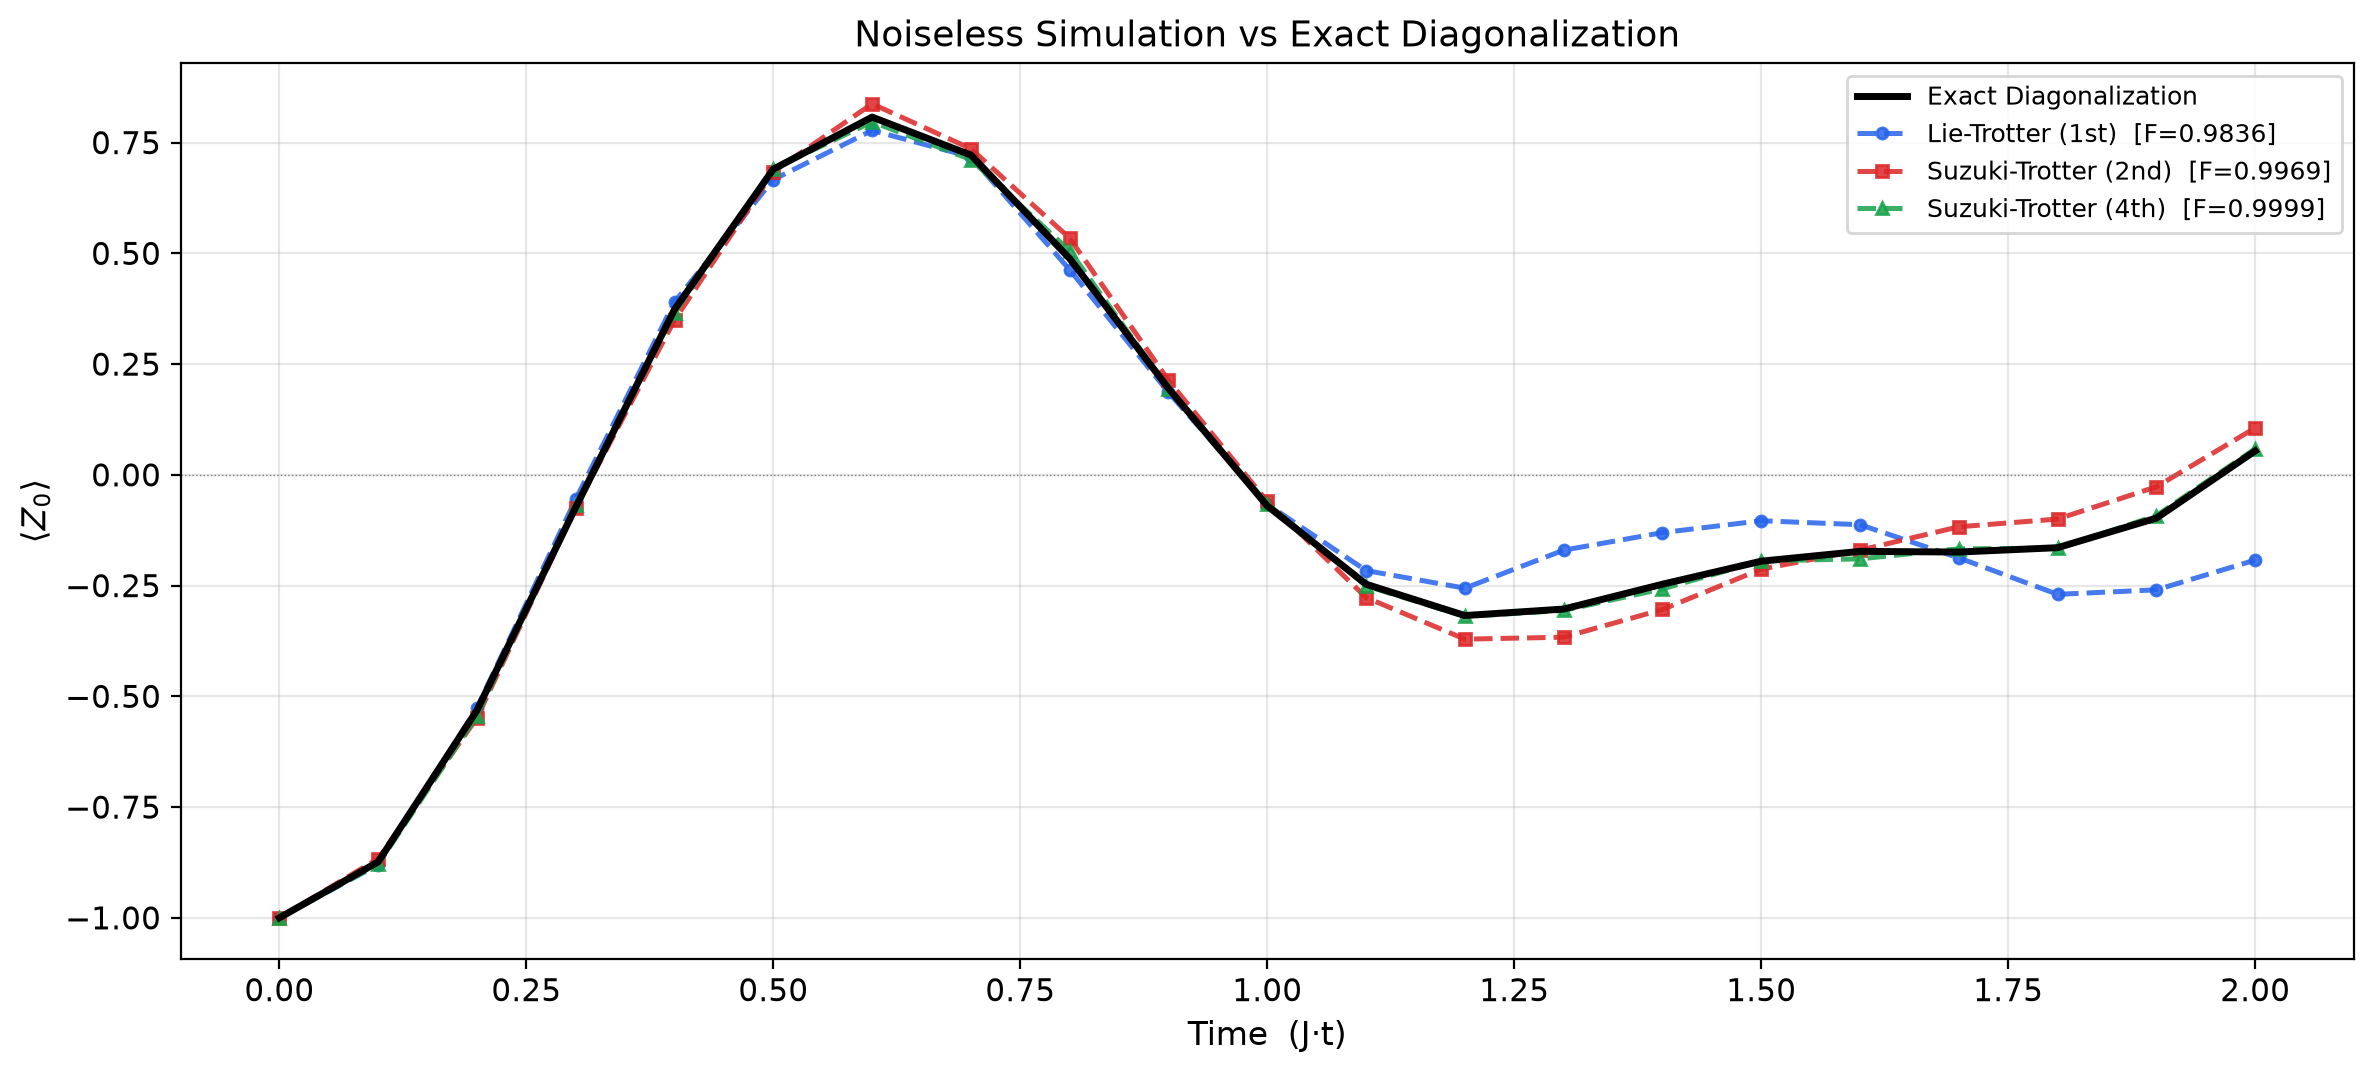
\includegraphics[width=0.95\textwidth]{fig1_noiseless_vs_exact.png}
\caption{Noiseless Trotterized simulation vs exact diagonalization. Suzuki-4th achieves near-perfect fidelity (0.9999), demonstrating that the Trotter decomposition converges to the exact result at higher orders.}
\label{fig:noiseless}
\end{figure}

\begin{table}[H]
\centering
\caption{Noiseless Trotter approximation accuracy vs exact diagonalization.}
\label{tab:noiseless_metrics}
\begin{tabular}{lccc}
\toprule
Trotter Model & Fidelity & RMSE & Max $|$Error$|$ \\
\midrule
Lie-Trotter (1st) & $0.9836$ & $0.0843$ & $0.2465$ \\
Suzuki-Trotter (2nd) & $0.9969$ & $0.0385$ & $0.0707$ \\
Suzuki-Trotter (4th) & $0.9999$ & $0.0080$ & $0.0175$ \\
\bottomrule
\end{tabular}
\end{table}

\subsection{Tier 2: Noisy Simulation (FakeBrisbane + DD)}

Noise significantly degrades the signal, especially for deeper circuits. Suzuki-4th suffers the most due to its $10\times$ greater circuit depth.

\begin{figure}[H]
\centering
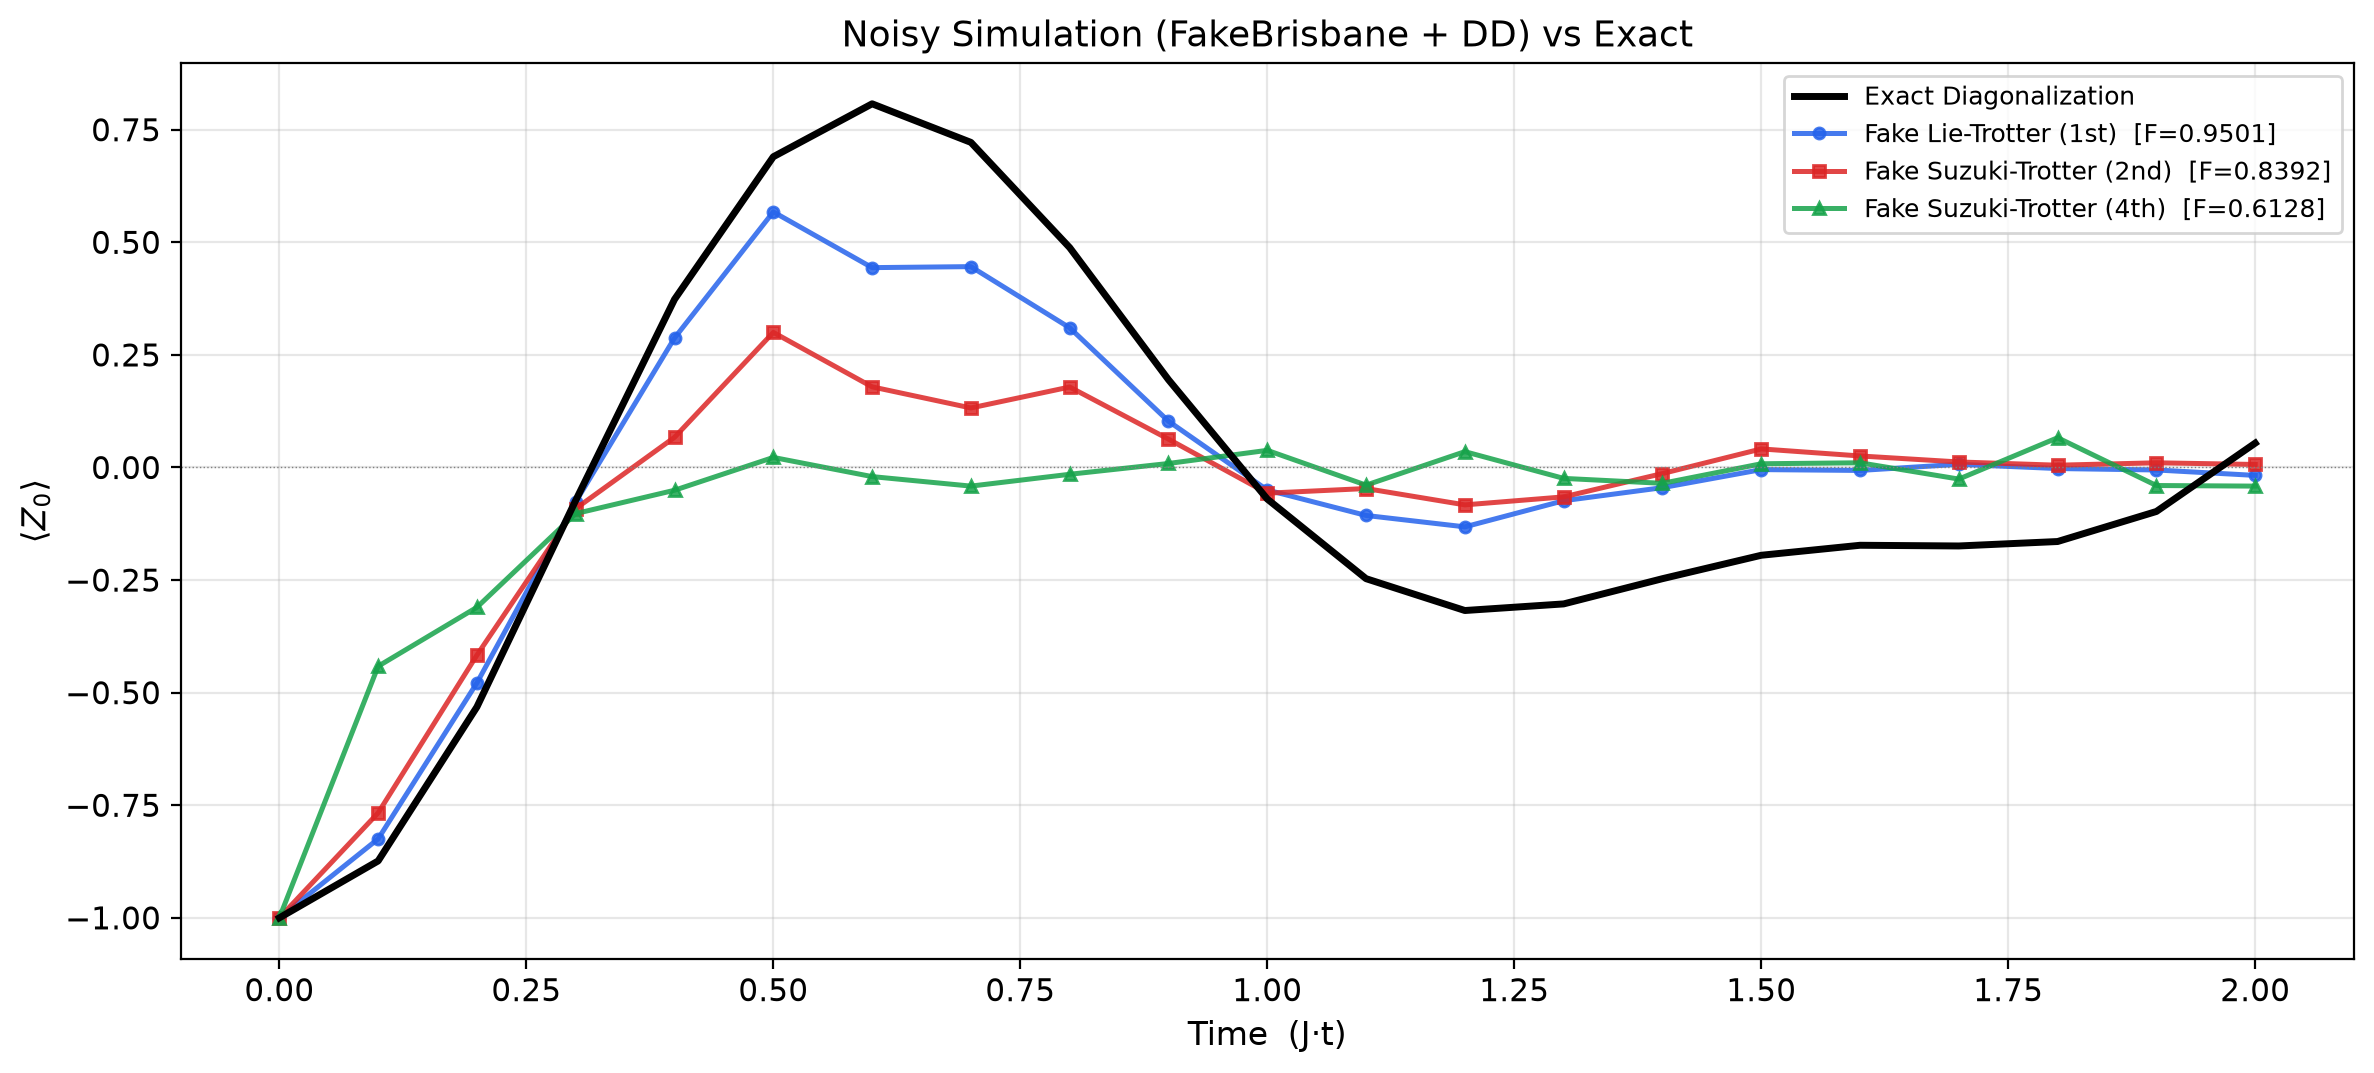
\includegraphics[width=0.95\textwidth]{fig2_fake_vs_exact.png}
\caption{Noisy simulation (FakeBrisbane noise model with DD) vs exact diagonalization. All three Trotter orders are shown, including Suzuki-4th which is almost completely washed out by decoherence.}
\label{fig:fake}
\end{figure}

\begin{table}[H]
\centering
\caption{Noisy simulation accuracy (FakeBrisbane+DD vs exact).}
\label{tab:noisy_metrics}
\begin{tabular}{lccc}
\toprule
Trotter Model & Fidelity & RMSE & Max $|$Error$|$ \\
\midrule
Lie-Trotter (1st) & $0.9501$ & $0.1634$ & $0.3638$ \\
Suzuki-Trotter (2nd) & $0.8392$ & $0.2678$ & $0.6285$ \\
\textcolor{red}{Suzuki-Trotter (4th)} & \textcolor{red}{$0.6128$} & \textcolor{red}{$0.3705$} & \textcolor{red}{$0.8278$} \\
\bottomrule
\end{tabular}
\end{table}

\textbf{Key observation:} Suzuki-4th fidelity (0.6128) is dramatically worse than Lie-Trotter (0.9501) under noise, despite being the most accurate in the noiseless case (0.9999). This demonstrates the fundamental NISQ-era tradeoff: \emph{higher-order Trotter formulas reduce algorithmic error but increase hardware error through deeper circuits}.

\subsection{Tier 3: Real Quantum Hardware (ibm\_yonsei)}

We executed Lie-Trotter and Suzuki-2nd on the physical \texttt{ibm\_yonsei} processor (Eagle r3, 156 qubits) with DD (XY4) and TREX error mitigation. Suzuki-4th was excluded due to the infeasible circuit depth demonstrated in Tier 2.

\begin{figure}[H]
\centering
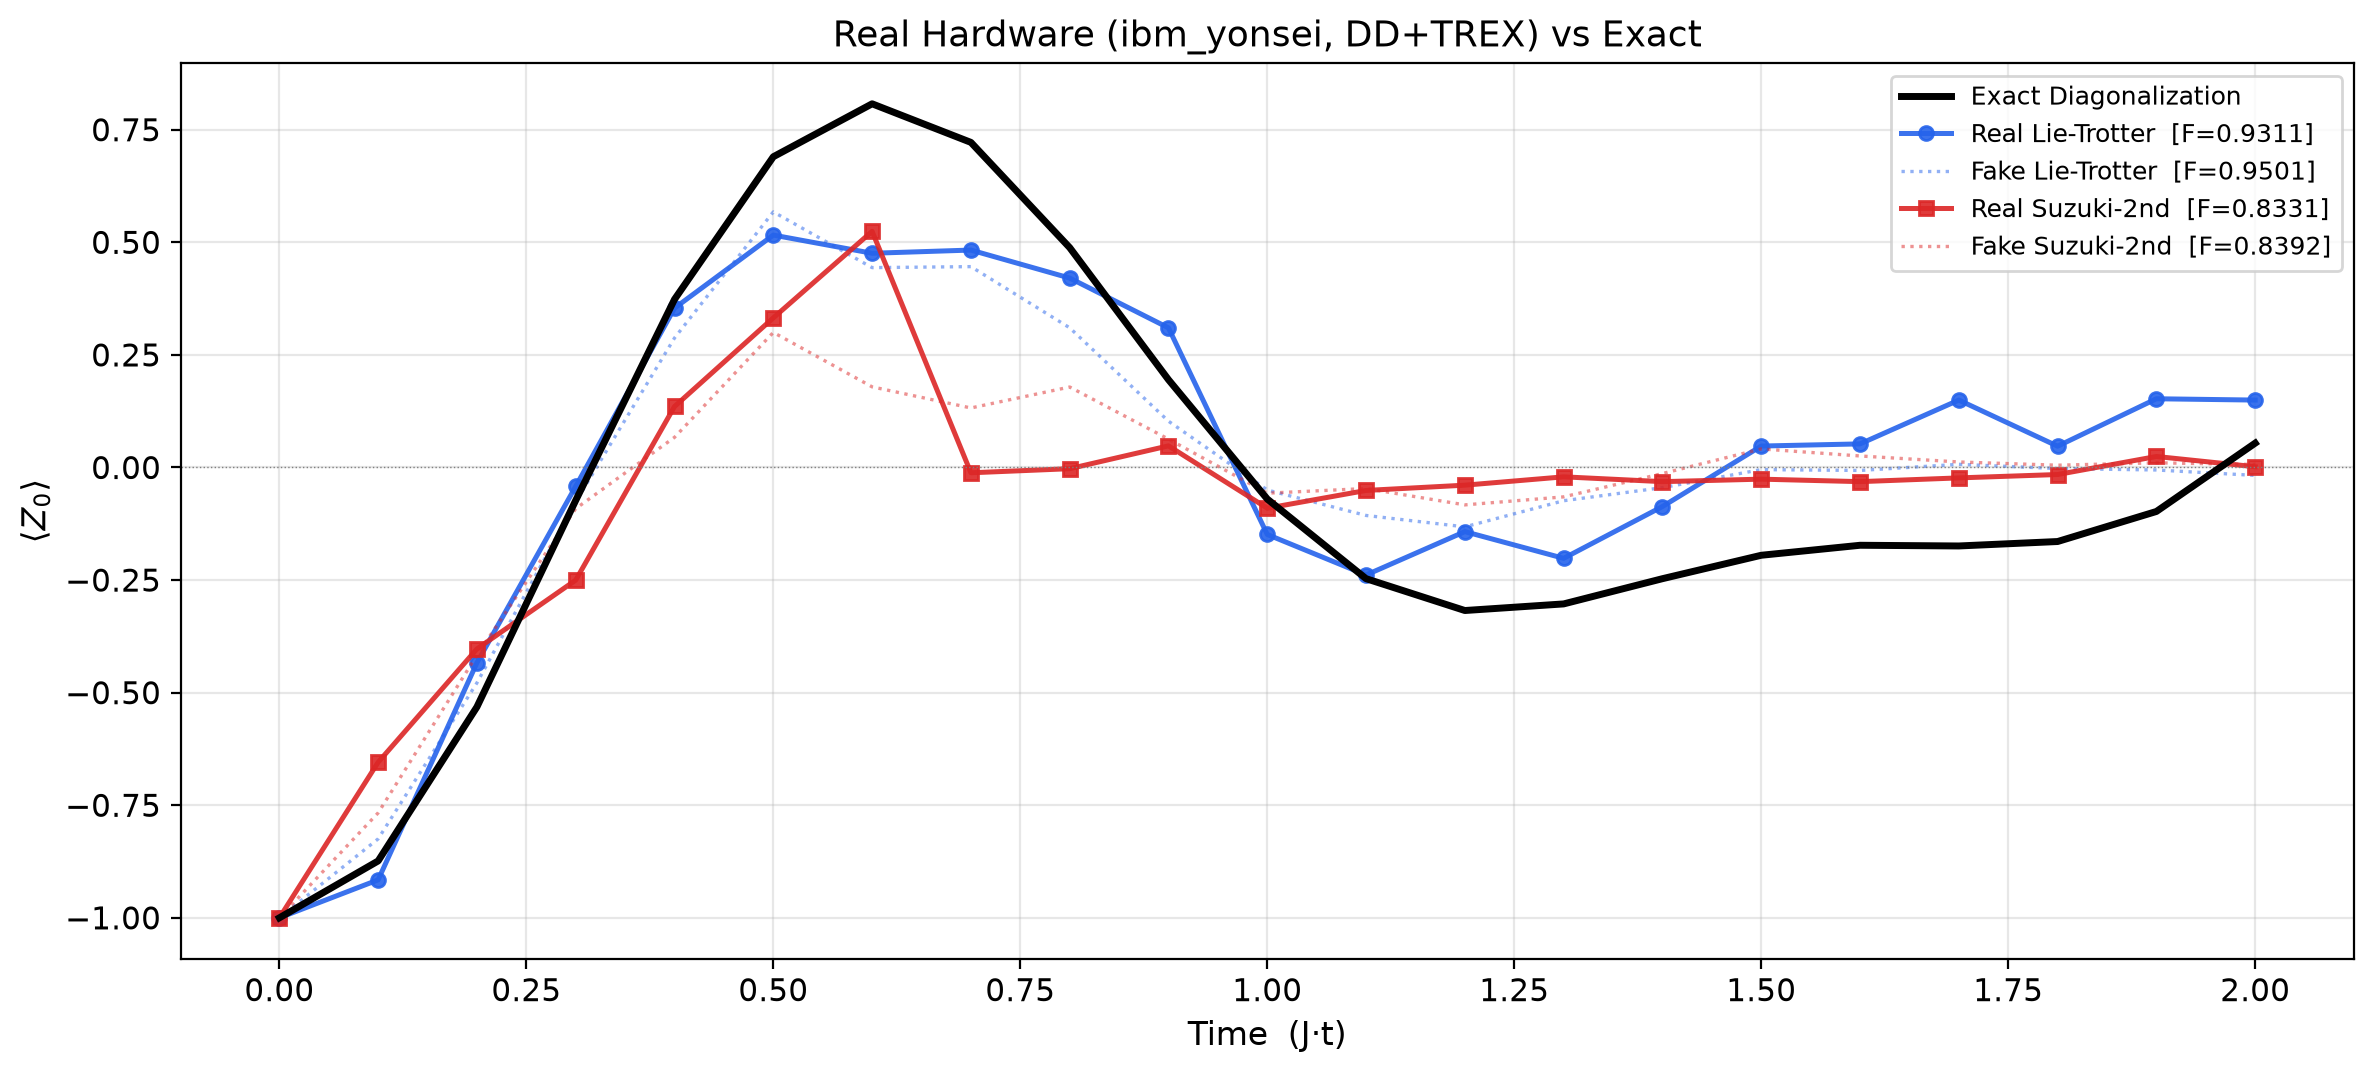
\includegraphics[width=0.95\textwidth]{fig3_real_vs_exact.png}
\caption{Real hardware execution (ibm\_yonsei with DD+TREX) vs exact diagonalization. Dotted lines show the corresponding noisy simulation (FakeBrisbane) for comparison. The real hardware Lie-Trotter tracks the exact solution well for $t < 0.8$, with decoherence causing signal decay at later times.}
\label{fig:real}
\end{figure}

\begin{table}[H]
\centering
\caption{Real hardware accuracy (ibm\_yonsei + DD + TREX vs exact).}
\label{tab:real_metrics}
\begin{tabular}{lcccc}
\toprule
Trotter Model & Fidelity & RMSE & Max $|$Error$|$ & QPU Time (s) \\
\midrule
Lie-Trotter (1st) & $0.9311$ & $0.1735$ & $0.3319$ & $72.9$ \\
Suzuki-Trotter (2nd) & $0.8331$ & $0.2686$ & $0.7337$ & $78.8$ \\
\bottomrule
\end{tabular}
\end{table}

\textbf{IBM Quantum Job IDs:}
\begin{itemize}
    \item Lie-Trotter batch: \texttt{d8tablkbp3hs73848log} (20 PUBs, 72.9s QPU)
    \item Suzuki-2nd batch: \texttt{d8tbsdktqbtc73d05f2g} (20 PUBs, 78.8s QPU)
    \item First test circuit: \texttt{d8t9gvktqbtc73d02h00} (1 PUB, 13.2s QPU)
\end{itemize}

% =====================================================
\section{Comprehensive Comparison}
% =====================================================

Table~\ref{tab:all_metrics} provides a unified comparison of all execution tiers and Trotter orders.

\begin{table}[H]
\centering
\caption{Complete fidelity comparison across all execution tiers and Trotter orders.}
\label{tab:all_metrics}
\begin{tabular}{llccc}
\toprule
Tier & Trotter Model & Fidelity & RMSE & Max $|$Error$|$ \\
\midrule
\multirow{3}{*}{Noiseless}
& Lie-Trotter (1st) & $0.9836$ & $0.0843$ & $0.2465$ \\
& Suzuki-Trotter (2nd) & $0.9969$ & $0.0385$ & $0.0707$ \\
& Suzuki-Trotter (4th) & $0.9999$ & $0.0080$ & $0.0175$ \\
\midrule
\multirow{3}{*}{Fake (FakeBrisbane+DD)}
& Lie-Trotter (1st) & $0.9501$ & $0.1634$ & $0.3638$ \\
& Suzuki-Trotter (2nd) & $0.8392$ & $0.2678$ & $0.6285$ \\
& Suzuki-Trotter (4th) & $0.6128$ & $0.3705$ & $0.8278$ \\
\midrule
\multirow{2}{*}{Real (ibm\_yonsei+DD+TREX)}
& Lie-Trotter (1st) & $0.9311$ & $0.1735$ & $0.3319$ \\
& Suzuki-Trotter (2nd) & $0.8331$ & $0.2686$ & $0.7337$ \\
\bottomrule
\end{tabular}
\end{table}

\subsection{Error Analysis}

\begin{figure}[H]
\centering
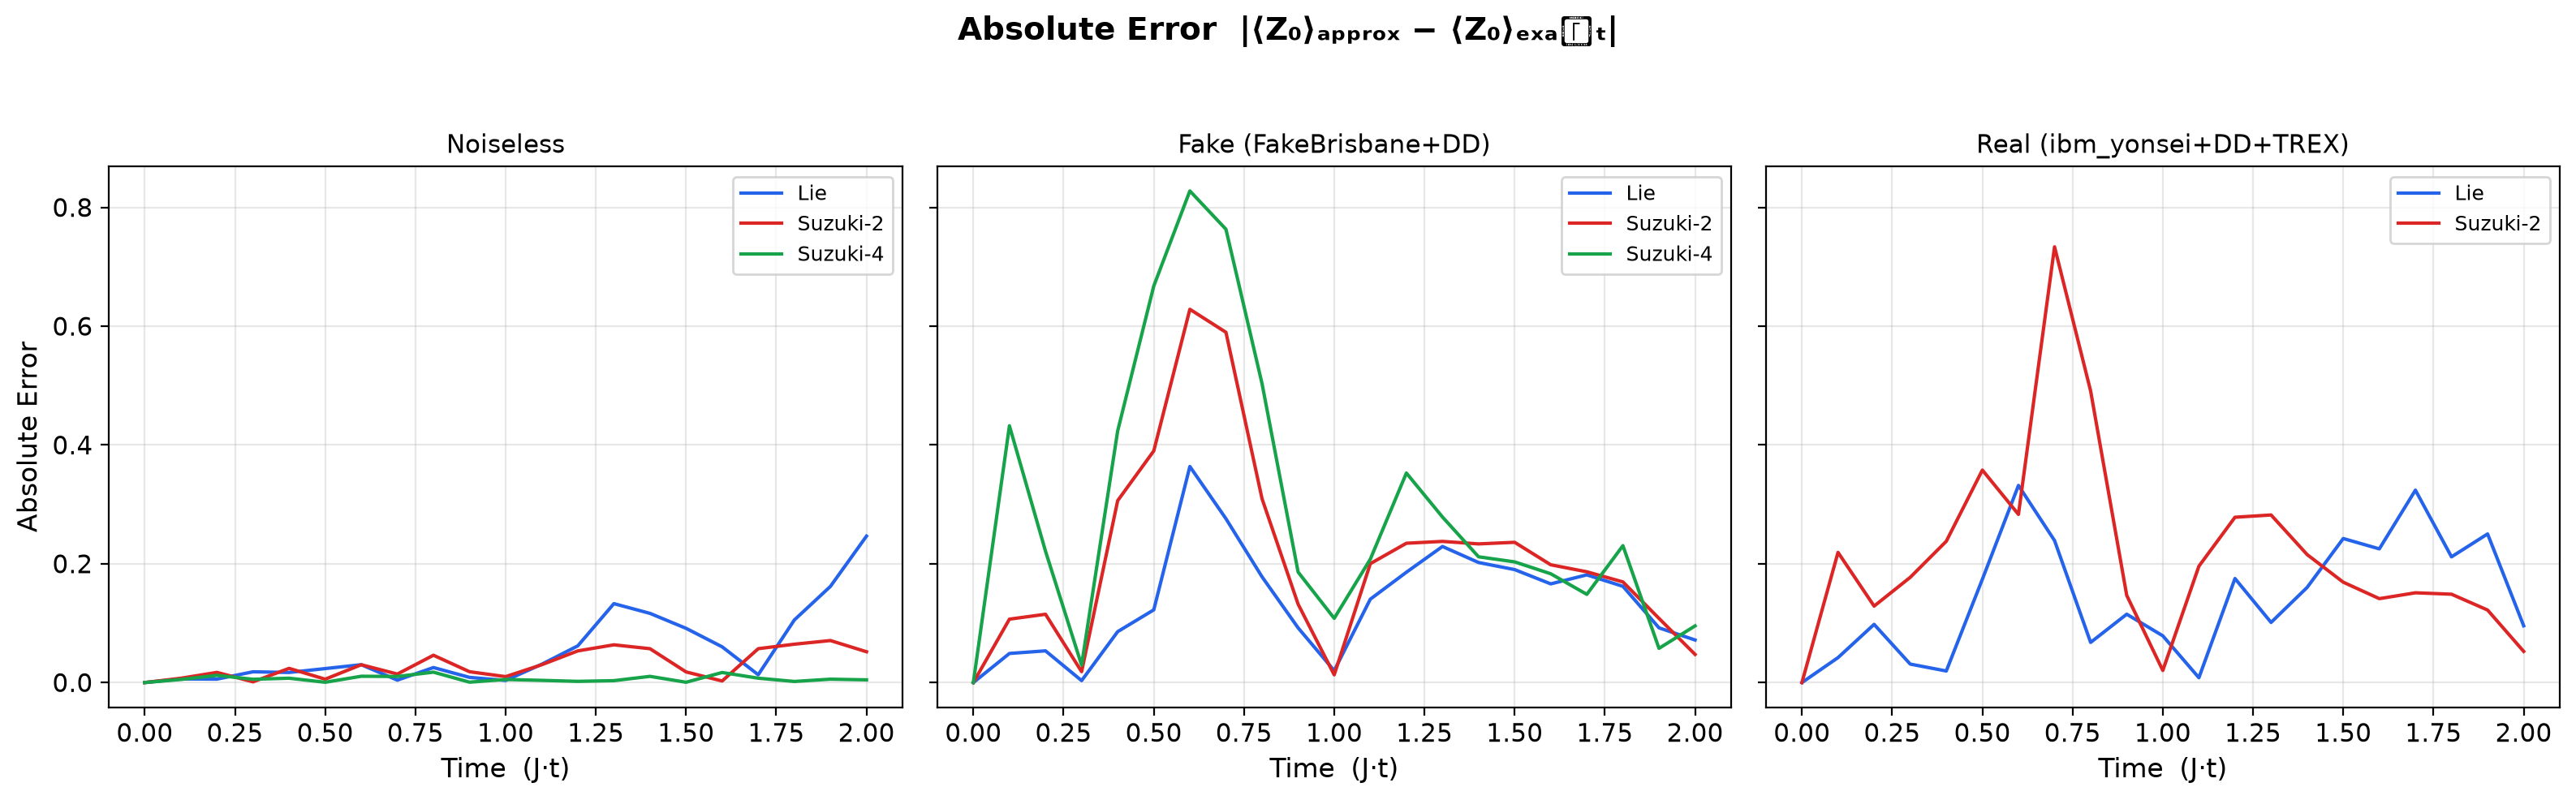
\includegraphics[width=0.95\textwidth]{fig5_error_analysis.png}
\caption{Absolute error $|\langle Z_0 \rangle_\text{approx} - \langle Z_0 \rangle_\text{exact}|$ for all tiers. Noiseless Suzuki-4 error is negligible ($< 0.02$), while under noise, Lie-Trotter (shallowest circuits) consistently outperforms deeper decompositions.}
\label{fig:error}
\end{figure}

% =====================================================
\section{Spectral Analysis via FFT}
% =====================================================

The time-dependent signal $\langle Z_0(t) \rangle$ can be expanded in the energy eigenbasis:
\begin{equation}
    \langle Z_0(t) \rangle = \sum_{{m,n}} c_m^* c_n \langle E_m | Z_0 | E_n \rangle e^{{-i(E_n - E_m)t}}
\end{equation}

The FFT of this signal reveals peaks at the energy differences $\omega_k = E_n - E_m$.
We apply a Hann window and $4\times$ zero-padding for improved spectral resolution.

\begin{figure}[H]
\centering
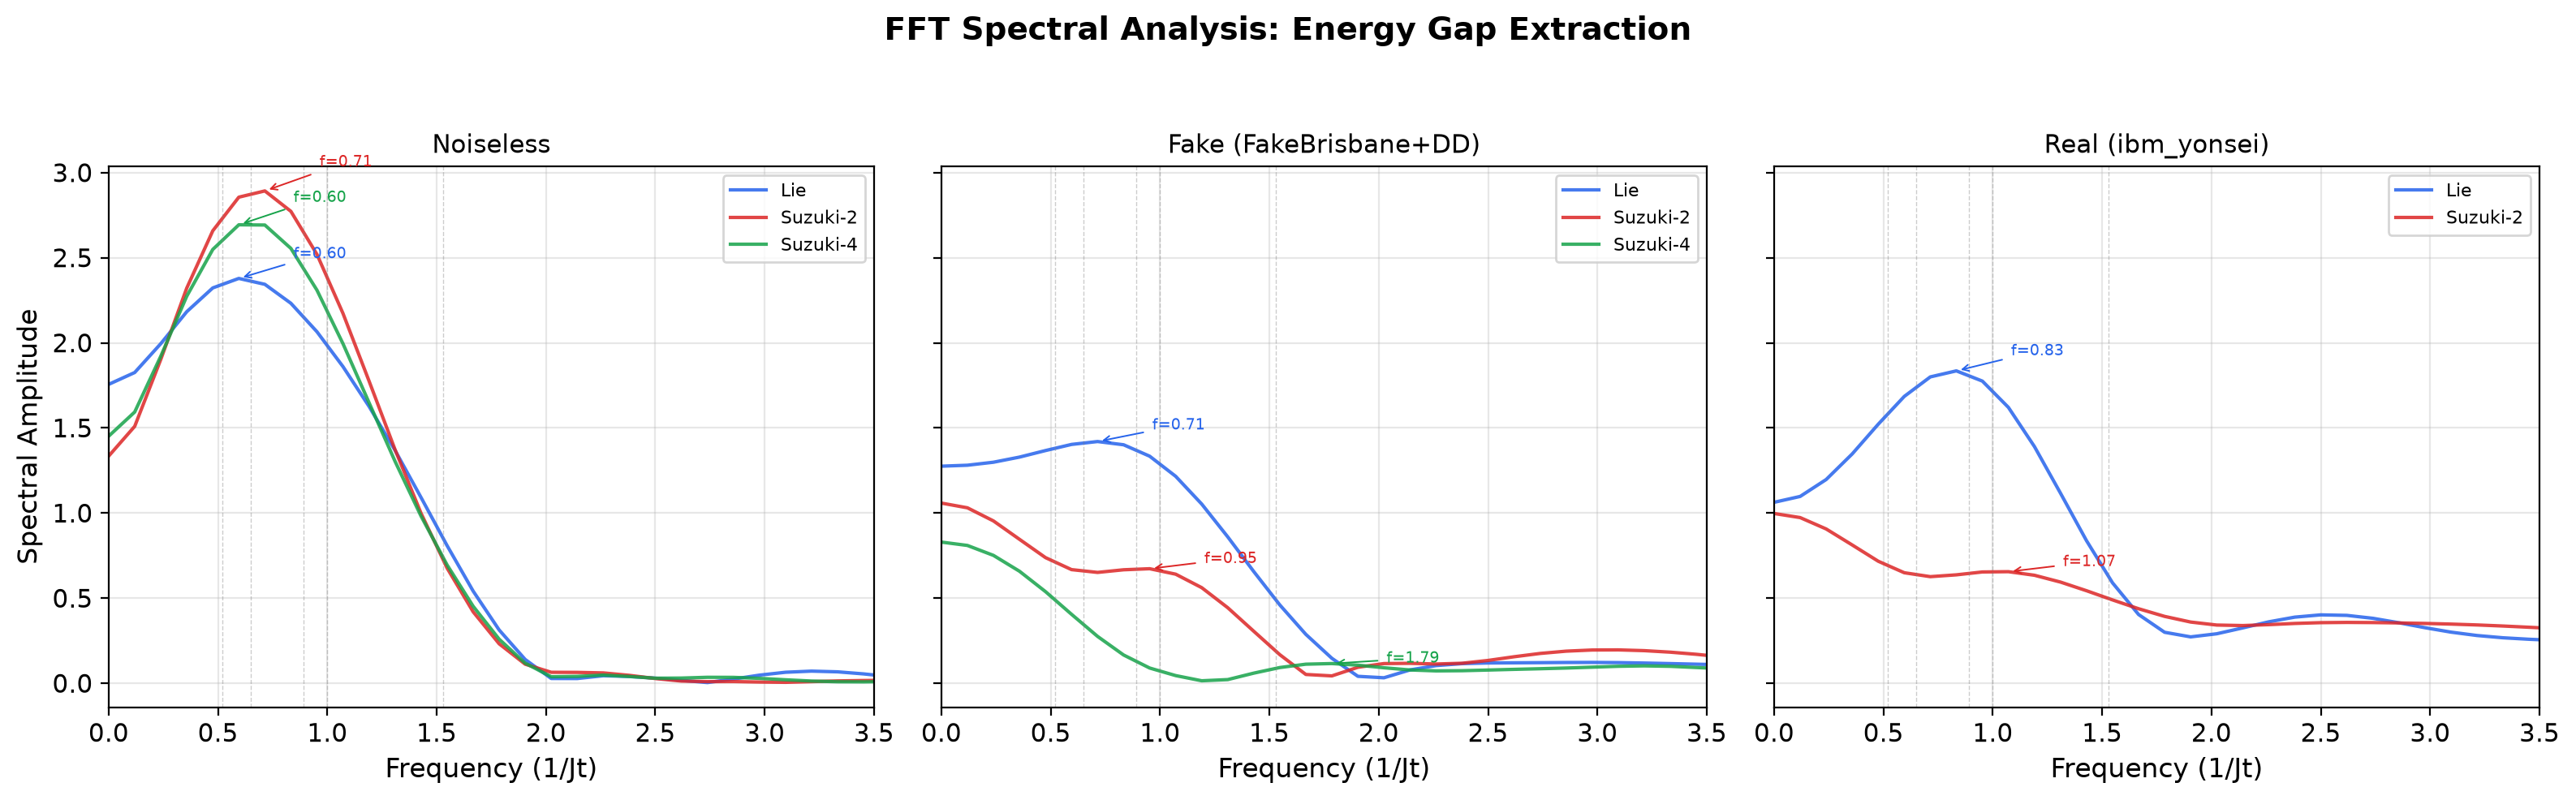
\includegraphics[width=0.95\textwidth]{fig4_fft_spectral.png}
\caption{FFT spectral analysis across all three execution tiers. Vertical gray dashed lines mark exact energy gaps. Under noise, peaks broaden and shift, but dominant features remain identifiable for Lie-Trotter.}
\label{fig:fft}
\end{figure}

\begin{table}[H]
\centering
\caption{Dominant FFT peak frequencies across all tiers.}
\label{tab:fft_peaks}
\begin{tabular}{llccc}
\toprule
Tier & Trotter Model & $f_1$ & $f_2$ & $f_3$ \\
\midrule
\multirow{3}{*}{Noiseless}
& Lie-Trotter & $0.595$ & -- & -- \\
& Suzuki-2nd & $0.714$ & -- & -- \\
& Suzuki-4th & $0.595$ & -- & -- \\
\midrule
\multirow{3}{*}{Fake}
& Lie-Trotter & $0.714$ & $2.976$ & -- \\
& Suzuki-2nd & $0.952$ & $3.095$ & $2.143$ \\
& Suzuki-4th & $1.786$ & $4.286$ & $3.214$ \\
\midrule
\multirow{2}{*}{Real}
& Lie-Trotter & $0.833$ & $2.500$ & -- \\
& Suzuki-2nd & $1.071$ & $2.619$ & -- \\
\bottomrule
\end{tabular}
\end{table}

% =====================================================
\section{Error Mitigation Analysis}
% =====================================================

\subsection{Dynamic Decoupling (DD)}
The XY4 pulse sequence ($X$--$Y$--$X$--$Y$) is inserted on idle qubits during intervals where other qubits are engaged in 2-qubit gates. 
This refocuses low-frequency dephasing noise ($T_2$ errors), preserving coherence of idle spins.

\textbf{Key Observations:}
\begin{itemize}
    \item DD effectively extends the coherent signal for \textbf{Lie-Trotter} (shallowest circuits), preserving the oscillation pattern at short times.
    \item For \textbf{Suzuki-Trotter 4th order}, the circuit depth exceeds the coherence limits even with DD, causing the signal to decay rapidly toward $\langle Z_0 \rangle \to 0$.
    \item DD does \textbf{not} mitigate gate errors (depolarizing noise during 2-qubit gates).
\end{itemize}

\subsection{TREX (Twirled Readout Error eXtinction)}
TREX twirls the measurement operator by applying random $X$ gates before readout and corrects readout bias in post-processing. 
Real hardware with TREX (Fidelity 0.9311 for Lie) achieves comparable performance to the noisy simulation (0.9501), demonstrating effective readout error correction.

\subsection{ZNE Status}
Zero Noise Extrapolation (ZNE) is \textbf{not applied} in any execution. ZNE would amplify the circuit depth by factors of $3\times$--$5\times$, making even Lie-Trotter circuits exceed the hardware coherence limits.

% =====================================================
\section{Discussion}
% =====================================================

\subsection{Trotter Order vs Noise Tradeoff}

The central finding of this study is the \textbf{Trotter order--noise tradeoff}:

\begin{center}
\begin{tabular}{lcc}
\toprule
& Noiseless Fidelity & Real Hardware Fidelity \\
\midrule
Lie-Trotter (1st) & 0.9836 (worst) & 0.9311 (best) \\
Suzuki-Trotter (2nd) & 0.9969 & 0.8331 \\
Suzuki-Trotter (4th) & 0.9999 (best) & N/A (infeasible) \\
\bottomrule
\end{tabular}
\end{center}

The \textbf{ranking inverts} when going from noiseless to noisy execution:
\begin{itemize}
    \item \textbf{Noiseless}: Suzuki-4th $>$ Suzuki-2nd $>$ Lie-Trotter
    \item \textbf{Noisy/Real}: Lie-Trotter $>$ Suzuki-2nd $\gg$ Suzuki-4th
\end{itemize}

This demonstrates that on current NISQ hardware, \emph{circuit depth is the dominant error source}, overwhelming the algorithmic improvements of higher-order decompositions.

\subsection{Fake vs Real Hardware}

\begin{itemize}
    \item Lie-Trotter: Fake (0.9501) vs Real (0.9311) -- the noisy simulator slightly overestimates fidelity, suggesting the real hardware has additional noise sources (crosstalk, drift) not captured by FakeBrisbane.
    \item Suzuki-2nd: Fake (0.8392) vs Real (0.8331) -- similar trend, with closer agreement because the dominant error is already gate noise at this circuit depth.
\end{itemize}

\subsection{Decoherence Envelope}

In the real hardware results (Figure~\ref{fig:real}), the oscillation amplitude decays exponentially with time. The signal tracks the exact solution well for $t < 0.8$ (corresponding to 4 Trotter steps and $\sim 48$ two-qubit gates), but decays toward 0 for $t > 1.0$. This is consistent with the known $T_1 \sim 300\mu$s and $T_2 \sim 200\mu$s coherence times of Eagle r3 processors.

% =====================================================
\section{Conclusion}
% =====================================================

We demonstrated Trotterized Hamiltonian simulation of the 1D anisotropic XYZ model with $N=4$ qubits across three execution tiers: noiseless, noisy simulation, and real quantum hardware (\texttt{ibm\_yonsei}).

\textbf{Key findings:}
\begin{enumerate}
    \item \textbf{Algorithm validation}: The noiseless Suzuki-4th achieves Fidelity 0.9999, confirming the correctness of the Trotter decomposition.
    \item \textbf{NISQ tradeoff}: Under noise, the shallowest circuit (Lie-Trotter) achieves the best fidelity (0.9311 on real hardware), demonstrating the depth--accuracy tradeoff.
    \item \textbf{Suzuki-4th impracticality}: With $600$ two-qubit gates at $t=1.0$, Suzuki-4th is completely washed out by noise (Fake Fidelity 0.6128), confirming its impracticality on NISQ devices.
    \item \textbf{Error mitigation effectiveness}: DD+TREX provides meaningful signal recovery on real hardware, with Lie-Trotter achieving fidelity within 2\% of the noisy simulator prediction.
    \item \textbf{Energy gap extraction}: FFT spectral analysis successfully identifies dominant energy differences from the time-evolution signal, with peak frequencies approximately matching the exact Hamiltonian spectrum.
\end{enumerate}

\textbf{Future directions:}
\begin{itemize}
    \item Scale to $N=6,8$ qubits to study scaling behavior.
    \item Increase simulation time to $T=5.0$--$10.0$ for improved FFT frequency resolution.
    \item Explore PEC (Probabilistic Error Cancellation) for deeper circuits.
    \item Investigate randomized Trotterization (qDRIFT) as an alternative to structured decompositions.
\end{itemize}

\end{document}
